%% Theorie.tex
%%
%\usepackage[ngerman]{babel}
%% ==============
\chapter{Theoretische Grundlagen}
\label{ch:Theorie}
%% ==============

%{\bibliographystyle{babalpha-fl}}	% german style
{\bibliographystyle{babunsrt-fl}}

Das Standardmodell der Teilchenphysik beschreibt die bisher bekannten fundamentalen Bausteine der Materie sowie deren Wechselwirkungen. In Kapitel \ref{ch:Theorie:sec:Standardmodell} wird ein kurzer \"Uberblick \"uber das Standardmodell gegeben. Auf die Produktion von Higgs-Boson und Topquark wird in Abschnitt \ref{ch:Theorie:sec:ttH} genauer eingegangen.\\


%% ===========================
\section{Das Standardmodell der Teilchenphysik}
\label{ch:Theorie:sec:Standardmodell}
%% ===========================

Der folgende Abschnitt soll einen kurzen \"Uberblick \"uber das Standardmodell der Elementarteilchenphysik geben, dabei bezieht er sich meist auf \cite{SWB-39819646X}.

Das Standardmodell der Elementarteilchenphysik ist eine Quantenfeldtheorie, in der die Theorie der elektroschwachen Wechselwirkung mit der Quantenchromodynamik zusammengefasst wird.\\% Das Universum besteht aus einigen grundlegenden Bausteinen, die durch vier elementare Kr\"afte beeinflusst werden \cite{O'Luanaigh:1997201}. Die bislang beste Beschreibung dieses Aufbaus liefert das Standardmodell, wenngleich es die vierte Kraft, die Gravitation, nicht erkl\"aren kann. Dennoch war es mit diesem Modell m\"oglich fast alle experimentellen Ergebnisse zu best\"atigen sowie sehr pr\"azise Vorhersagen \"uber verschiedene Ph\"anomene zu treffen.
Das Standardmodell liefert die bislang beste Beschreibung der bisher bekannten grundlegenden Bestandteile des Universums und der vier Kr\"afte, die diese beeinflussen, wenngleich die vierte Kraft, die Gravitation, nicht vom Standardmodell erkl\"art werden kann. Die drei im Standardmodell beschriebenen elementaren Kr\"afte sind starke und schwache Wechselwirkung sowie die elektromagnetische Wechselwirkung. Der elektromagnetischen Wechselwirkung unterliegen alle Teilchen, die eine elektrische Ladung besitzen. Die Ladung der schwachen Wechselwirkung wird schwache Ladung genannt. In Analogie zur Farbmischung nennt man die Ladungen der starken Wechselwirkung Farbladungen, da sich die drei verschiedenen Farbladungen (rot, gr\"un und blau) zur neutralen Ladung addieren. Trotz der im Modell fehlenden Gravitation war es mit diesem Modell m\"oglich, fast alle experimentellen Ergebnisse zu best\"atigen sowie sehr pr\"azise Vorhersagen \"uber verschiedene Ph\"anomene zu treffen.

%Die drei im Standardmodell beschriebenen elementaren Kr\"afte sind starke und schwache Wechselwirkung sowie die elektromagnetische Wechselwirkung. Der elektromagnetischen Wechselwirkung unterliegen alle Teilchen, die eine elektrische Ladung besitzen. Die Ladung der schwachen Wechselwirkung wird schwache Ladung genannt. In Analogie zur Farbmischung nennt man die Ladungen der starken Wechselwirkung Farbladungen, da sich die drei verschiedenen Farbladungen (rot, gr\"un und blau) zur neutralen Ladung addieren.

Die bislang entdeckte Materie besteht aus zwei Arten von Elementarteilchen, den Leptonen und den Quarks. Diese lassen sich jeweils in drei Familien unterteilen. Jede Quark-Familie besteht jeweils aus einem Quarkpaar und deren Antiteilchen. Sie bestehen aus Up- und Down-, Strange- und Charm- sowie Bottom- und Topquark.\\
Leptonen bilden jeweils zusammen mit dem dazugeh\"origen Neutrino und den jeweiligen Antiteilchen eine Familie. Im Gegensatz zu den Quarks unterliegen Leptonen nicht der starken Wechselwirkung.\\
%Die dritte elementare Wechselwirkung, die im Standardmodell beschrieben ist, ist die elektromagnetische Wechselwirkung. Ihr unterliegen alle geladenen Teilchen. Diese Wechselwirkungen sind in ihrer Struktur sehr \"ahnlich und werden durch den Austausch von Vektorbosonen vermittelt. Diese sind die Gluonen der starken Wechselwirkung, die W- und Z-Bosonen der schwachen Wechselwirkung und die Photonen ($\gamma$) der elektromagnetischen. W\"ahrend die Fermionen aus denen die Materie besteht, einen halbzahligen Spin besitzen, haben die Bosonen einen ganzzahligen Spin.
Die drei elementaren Wechselwirkungen des Standardmodells sind in ihrer Struktur sehr \"ahnlich und werden durch den Austausch von Vektorbosonen vermittelt. Diese sind die Gluonen der starken Wechselwirkung, die W- und Z-Bosonen der schwachen Wechselwirkung und die Photonen ($\gamma$) der elektromagnetischen Wechselwirkung.% W\"ahrend die Fermionen aus denen die Materie besteht, einen halbzahligen Spin besitzen, haben die Bosonen einen ganzzahligen Spin.

Der letzte fehlende Baustein im Standardmodell ist ein elementares Spin-0-Teilchen, ohne das keine konsistente Erkl\"arung f\"ur die W- und Z$^0$-Massen m\"oglich w\"are. Dieses ist das Higgs-Boson, welches 2012 am CERN entdeckt wurde \cite{Chatrchyan201230}\cite{Aad20121}. Die Kopplung zwischen Higgs-Boson und Fermionen ist proportional zur Fermionenmasse.

In Abbildung \ref{fig:Standardmodell} sind alle elementaren Bosonen und Fermionen dargestellt. Jeder Eintrag steht f\"ur ein Elementarteilchen. In der Mitte ist jeweils gro\ss~das Symbol f\"ur das Teilchen dargestellt, darunter der vollst\"andige Name. Die erste Zahl in der linken oberen Ecke jedes Eintrags gibt die Ruhemasse des Teilchens an. Darunter stehen elektrische Ladung in Einheiten der Elementarladung und der Spin des Teilchens. Die Fermionen werden in Quarks (lila) und Leptonen (gr\"un) unterteilt. Jede Spalte entspricht einer Fermionenfamilie oder Generation. In rot sind die Eichbosonen der grundlegenden Wechselwirkungen des Standardmodells dargestellt, in gelb das Higgs-Boson.

\begin{figure}[hhh]
 \begin{center}
   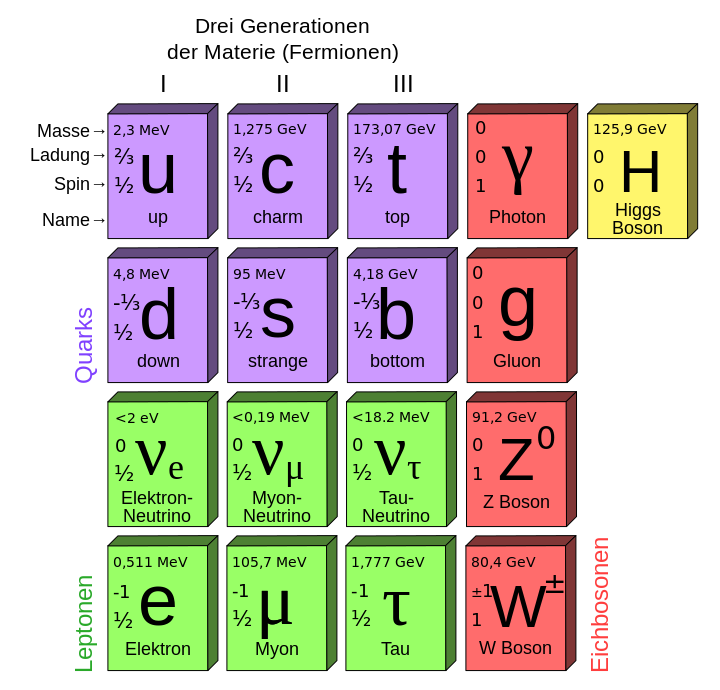
\includegraphics[width=\textwidth]{graphics/Standard_Model.png}
   \parbox[b]{12cm}{
     \caption[Standardmodell der Teilchenphysik]
             {\label{fig:Standardmodell}\it Die 12 fundamentalen Fermionen und f\"unf fundamentalen Bosonen des Standardmodells der Teilchenphysik,\\ Quelle: \cite{wiki:Standardmodell}}
   }
 \end{center}
\end{figure}

Insgesamt stimmen die experimentellen Ergebnisse gut mit den Vorhersagen des Standardmodells \"uberein. Dennoch reicht das Modell nicht aus, um s\"amtliche Ph\"anomene zu erkl\"aren. Im Modell werden beispielsweise masselose Neutrinos gefordert, allerdings ist durch die Beobachtung von Neutrinooszillationen erwiesen, dass massive Neutrinos existieren.

%% ===========================
\section{Assoziierte Higgs-Boson-Top-Quark-Paar-Produktion (\ttH)}
\label{ch:Theorie:sec:ttH}
%% ===========================

%Da die Kopplungskonstante zwischen Higgs-Boson und Fermionen im Standardmodell von der Fermionenmasse abh\"angt, ist eine Untersuchung der Kopplung zwischen Top-Quark und Higgs-Boson aufgrund der hohen Masse des Top-Quarks verglichen mit anderen Quarkmassen, besonders interessant. In Tabelle \ref{tab:quarkmasse} sind zum Vergleich die Quarkmassen aufgelistet.\\
Die Kopplungen zwischen Fermionen und dem Higgs-Boson nennt man Yukawa-Kopplungen.
Sie sind im Standardmodell freie Parameter, die experimentell bestimmt werden m\"ussen. Da sie von den Fermionenmassen abh\"angen, ist eine Untersuchung der Kopplung zwischen Top-Quark und Higgs-Boson aufgrund der hohen Masse des Top-Quarks, verglichen mit anderen Quarkmassen, besonders interessant. In Tabelle \ref{tab:quarkmasse} sind die Quarkmassen aufgelistet.\\

\begin{table}[hhh]\parbox{12cm}{
  \caption[Quarkmassen]{\it Quarkmassen {\rm \cite{Agashe:2014kda}}
  }\label{tab:quarkmasse}}
  \begin{center}
  \begin{tabular}{lll}
  \hline
  {\bf Quark} & {\bf Symbol} & {\bf Masse}  \\
  \hline \hline
     %Up		& u & \num{2,3}$^{+0,7}_{-0,5}$ \\
     %Down	& d & $4,8^{+0,5}_{-0,3}$~MeV\\
     %Strange& s & $95\pm 5$~MeV \\
     %Charm	& c & $1,275\pm 0,025$~GeV \\ 
  	 %Bottom & b & $4,18\pm 0,03$~GeV \\
     %Top    & t & $ 173,07\pm 0,52\pm 0,72$~GeV \\  
     Up		& u & $\num{2,3}^{{+0,7}}_{{-0,5}}\si{\mega\electronvolt}$ \\
     Down	& d & $\num{4,8}^{{+0,5}}_{{-0,3}}\si{\mega\electronvolt}$ \\
     Strange& s & $\num{95}\pm \num{5}\si{\mega\electronvolt}$ \\
     Charm	& c & $\num{1,275}\pm \num{0,025}\si{\giga\electronvolt}$ \\ 
  	 Bottom & b & $\num{4,18}\pm \num{0,03}\si{\giga\electronvolt}$ \\
     Top    & t & $\num{173,07}\pm \num{0,52}\pm \num{0,72}\si{\giga\electronvolt}$\\                                
  \hline
  \end{tabular}
  \end{center}
\end{table}

Die Kopplung zwischen Top-Quark und Higgs-Boson kann im Prozess der assoziierten Produktion eines Higgs-Bosons mit einem Paar aus Top-Quark und Top-Anti-Quark (\ttH) untersucht werden.\\
Wechselwirkungen zwischen Teilchen k\"onnen durch Feynman-Diagramme visualisiert werden. In Abbildung \ref{fig:ttH_feynmans} sind exemplarisch einige Feynman-Diagramme zur \ttH-Produktion in f\"uhrender Ordnung abgebildet.% und zum Vergleich das Feynman-Diagramm der Gluon-Gluon-Fusion, des dominierenden Kanals der Higgs-Boson-Produktion am LHC, in Abbildung \ref{fig:gluonfusion}.
In Abbildung \ref{fig:gluonfusion} ist zum Vergleich das Feynman-Diagramm der Gluon-Gluon-Fusion, des dominierenden Kanals der Higgs-Boson-Produktion am LHC abgebildet.
%Diese Kopplung kann w\"ahrend der assoziierten Produktion eines Higgs-Bosons mit einem Paar aus Top-Quark und Top-Anti-Quark untersucht werden.\\
%Wechselwirkungen zwischen Teilchen k\"onnen durch Feynman-Diagramme visualisiert werden. In Abbildung \ref{fig:ttH_feynmans} sind exemplarisch einige Feynmandiagramme zur \ttH-Produktion in f\"uhrender Ordnung abgebildet.

%\begin{figure}[hhh]
% \begin{center}
%   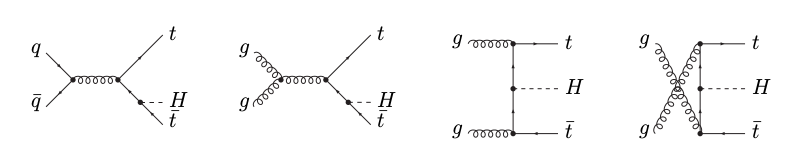
\includegraphics[width=\textwidth]{graphics/ttH_feynmans.png}
%   \parbox[b]{12cm}{
%     \caption[\ttH Feynman-Diagramme]
%             {\label{fig:ttH_feynmans} {\label{fig:gluonfusion} \it\!Feynman-Diagramm f\"ur die Gluon-Gluon-Fusion, den dominierenden Kanal der Higgs-Boson-Produktion am LHC, erstellt mit \cite{feynman_draw}}}}
             %\it Feynman-Diagramme f\"ur die \ttH-Produktion aus Hadronenkollisionen in f\"uhrender Ordnung \cite{hep-ph/0211352}}
% \end{center}
%\end{figure}

 \begin{figure}[hhh]
  \begin{center}
    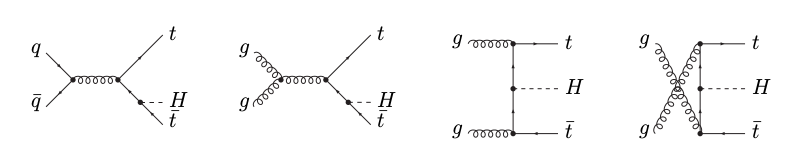
\includegraphics[width=\textwidth]{graphics/ttH_feynmans.png}
    \parbox[b]{12cm}{
      \caption[\ttH Feynman-Diagramme]
             {\label{fig:ttH_feynmans} \it\!Feynman-Diagramme f\"ur die \ttH-Produktion aus Hadronenkollisionen in f\"uhrender Ordnung \cite{hep-ph/0211352}}
   }
 \end{center}
\end{figure}


 \begin{figure}[hhh]
  \begin{center}
    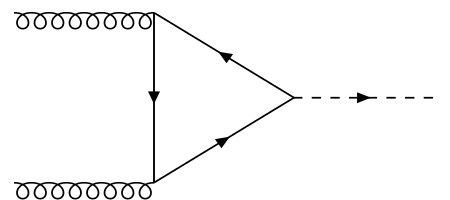
\includegraphics[width=0.4\textwidth]{graphics/gluonfusion.png}
    \parbox[b]{12cm}{
      \caption[Gluon-Gluon-Fusion Feynman-Diagramm]
             {\label{fig:gluonfusion} \it\!Feynman-Diagramm f\"ur die Gluon-Gluon-Fusion, den dominierenden Kanal der Higgs-Boson-Produktion am LHC, erstellt mit \cite{feynman_draw}}
    }
  \end{center}
 \end{figure}